As discussed in section \ref{sec:StateOfTheArt}, the TRITIUM consists in a chain of three main elements:

\begin{itemize}

\item{} The scintillator, that detects the tritium event, as ionizing radiation hits this material and deposits kinetic energy through ionization and excitation processes, part of the absorbed energy is converted in to photons, mostly in the visible range\footnote{The visible range is made up by photons with a wavelength between $380~\nm$ and $750~\nm$}. The produced photons carry information about the particle detected, like its energy, type, etc.

\item{} The photosensor, that detects the photons produced in the scintillator. The most common photosensors in nuclear physics are PMTs and SiPMs. They detect the photons produced in the scintillator with an efficiency and transforms them in electrons with a multiplication factor of around $10^6$. These electrons form a electronic pulse than gives information of the detected photons.

\item{} The electronic system, which is the part of the scintillator detector in charge of processesing and analyzing (first analogically and then digitally) the electrical pulse given by the photosensor. The output of the electronic system is the useful information about the events detected such as number and energy spectrum.

\end{itemize}

In Figure \ref{fig:ScintillatorDetector} a scheme of a scintillation detector is shown. There, the scintillator detects ionizing radiation and produces photons that are guided by the reflector and the light guide to the photosensor. Some of the photons that reach the sensitive part of the photosensors are converted and multiplied, forming a electronic pulse. The output signal of the photosensor (electronic pulse) is processed and analyzed by the corresponding electronics:

\begin{figure}[hbtp]
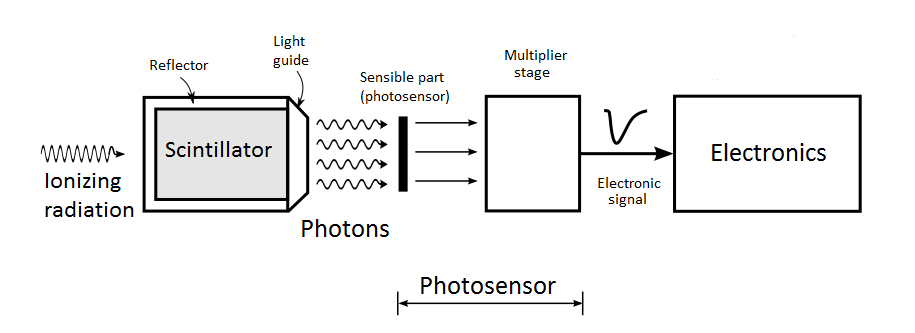
\includegraphics[scale=0.6]{3DesignPrinciples/32Tritium_detector/ScintillatorDetector.png}
\centering
\caption{Scheme of the scintillator detector\label{fig:ScintillatorDetector}}
\end{figure}
